\section{Probability and Statistics}

\textit{Most of the material covered in this section is also covered in my MATH 318 notes.}

\subsection{Permutations}

Permutations are combinations where order matters. How permutations are calculated depends on whether repetitions are allowed or not. The number of permutations made from choosing $k$ from $n$ items when repetitions are allowed is $n^k$. \\

When repetitions are not allowed, the number of permutations is just $n!$. Here is one way to understand where this formula came from: For the first item, there are $n$ choices to place and since no repetitions are allowed, there are $n-1$ choices left for the second item and so on.

\begin{texample}
	Calculate the probability of obtaining exactly $k=3$ heads and tails for a total of 6 coin tosses. \\
	
	There are the total of $2^6=64$ possible outcomes. The number of times when the combination $HHHTTT$ occurs is $\frac{6!}{3!3!}=20$. Therefore the probability is $\frac{20}{64}=\frac{5}{16}$. \\
	
	For $k$ values larger than $3$, the probability of getting the equal number of heads and tails will be low. It will be close to zero as $k \to \infty$.
\end{texample}

\begin{texample}
	Find the number of words created from rearranging letters $ALLELE$. \\
	
	There are two $E$s and three $L$s. Notice that there is no difference when you reorder these letters. Each word created from two $E$s and three $L$s corresponds to $2!3!$ permutations. \\
	
	The number of permutations is $6!$ which includes duplicates. To get the final answer, we divide it by $2!3!$ which gives $\frac{6!}{2!3!}=60$ total words. \\
	
	Speaking of probability, there are no arrangements of $ALLELE$ that is more likely than others. This makes $ALLLEE$ equally likely.
\end{texample}

To calculate the number of permutations made from choosing $k$ out of $n$ items with no repetition:

$$n(n-1)(n-2) \cdots (n-k+1)=\frac{n!}{(n-k)!}$$

It is usually denoted by ${}_n \mathrm{P}_k$.

\subsection{Combinations}

\begin{texample}
	How many ways to pick two out of $\{a, b, c, d\}$? \\
	
	Initially, there are four choices for the first letter of a ordered pair. After picking one, there are three choices left. There are $4(3)=12$ ordered pairs: $ab, ba, ac, ca, ad, da, bc, cb, bd, db, cd, dc$. However, we don't care about the order (ie. $ab$ and $ba$ is considered the same) so we divide by $2!$ which gives: $\frac{12}{2}=6$ combinations.
\end{texample}

To pick $k$ out of $n$ items, the total number of combinations is the number of ways to create ordered combinations (permutations) of size $k$ divided by the number of permutations of $k$ items in combinations. The calculation process is outlined below:

\begin{align*}
	\frac{n(n-1)(n-2) \cdots (n-k+1)}{k!} = \frac{\frac{n!}{(n-k)!}}{k!} = \frac{n!}{k!(n-k)!}
\end{align*}

We use $\binom{n}{k}$ to denote $\frac{n!}{k!(n-k)!}$. It is read as ``n choose k.'' This is a binomial coefficient. Another way to think about combinations is that it is the same as finding how many ways to rearrange $n$ cards where $k$ cards are coloured red and $n-k$ cards are coloured green. Also note that:

\begin{align*}
	\binom{n}{n-k} = \frac{n!}{(n-k)!(n-(n-k))!} = \frac{n!}{(n-k)!k!} = \binom{n}{k}
\end{align*}

$\binom{n}{k}$ makes a Gaussian curve as shown below.

\begin{figure}[H]
	\centering
	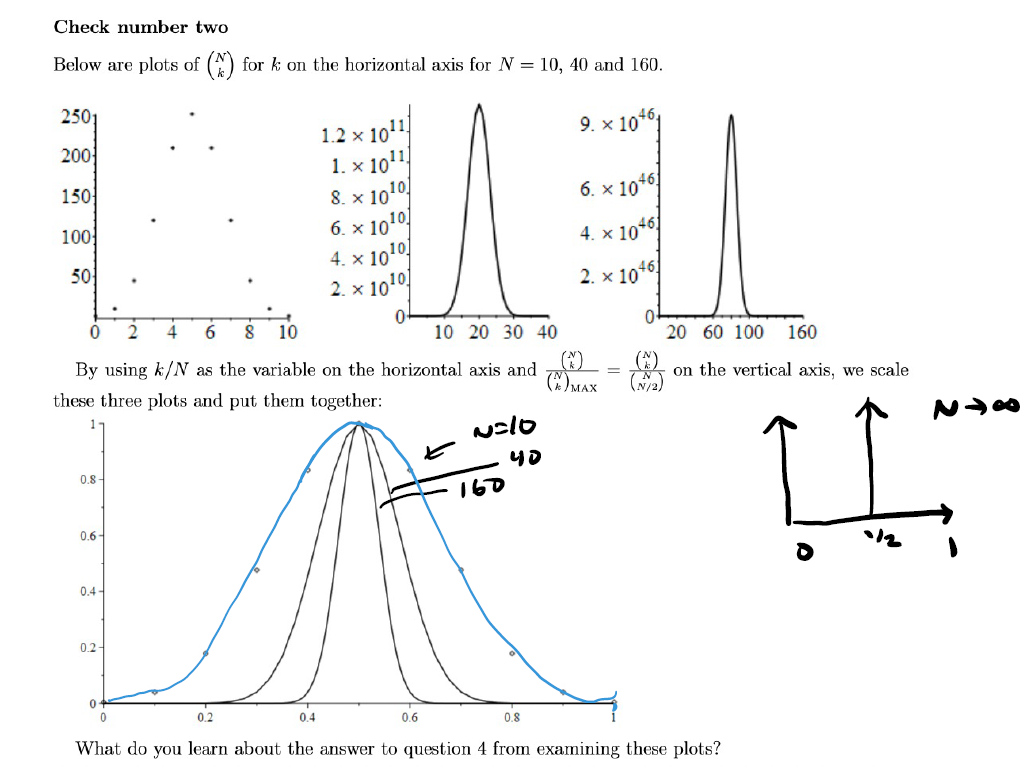
\includegraphics[width=160mm]{1.png}
	\caption{Gaussians for different $N$}
\end{figure}

$\binom{n}{k}$ is maximized when $k=n/2$. \\

There is an interesting observation that can be used to calculate binomial coefficients. Suppose you toss a coin $n$ times and $k$ of $n$ tosses are heads. The number of possible ways to get $k$ heads out of $n$ tosses is given by $\binom{n}{k}$. To find this binomial coefficient, consider two cases: the first toss is H and the first toss is not H. When the first toss is H, the remaining tosses $n-1$ must have $k-1$ heads and the number of possible ways it can happen is $\binom{n-1}{k-1}$. When the first toss is not H,  the remaining tosses $n-1$ must have $k$ heads and the number of possible ways it can happen is $\binom{n-1}{k}$. The number of possible ways to get $k$ heads out of $n$ tosses is the number of possible ways to get H as the first toss plus the number of possible ways not to get H as the first toss:

$$\binom{n}{k} = \binom{n-1}{k-1} + \binom{n-1}{k}$$

This is called ``Pascal's rule.'' It can be used to construct Pascal's triangle.

\begin{center}
	\begin{tabular}{rccccccccc}
		&    &    &    &    &  1\\\noalign{\smallskip\smallskip}
		&    &    &    &  1 &    &  1\\\noalign{\smallskip\smallskip}
		&    &    &  1 &    &  2 &    &  1\\\noalign{\smallskip\smallskip}
		&    &  1 &    &  3 &    &  3 &    &  1\\\noalign{\smallskip\smallskip}
		&  1 &    &  4 &    &  6 &    &  4 &    &  1\\\noalign{\smallskip\smallskip}
	\end{tabular}
\end{center}

$\binom{n}{k}$ gives the value at $n$th row and $k$th column (both zero-indexed) of the triangle. For example, in the third row and second column, $\binom{2}{1}=2$. Notice that the total in each row is always $2^n$.

\subsection{Frequentist Definition of Probability}

Consider an experiment with distinct outcomes $O_1, O_2, \dots, O_i$. Repeat this experiment $N$ times. Let $N_i$ be the number of times outcome $O_i$ occurs (out of $N$). Probability $P(O_i)$ of $O_i$ is given by:

$$P(O_i) = \lim_{N \to \infty} \frac{N_i}{N}$$

If we know that the probability of some event $E$ is $P(E)$, our best prediction for how many times we will see event $E$ occur out of $n$ attempts is $nP(E)$.

\subsection{Example: Coin Toss Experiment}

Consider an experiment where a fair coin is tossed $k$ times. We repeat this process for $N$ times. We define score is the number of heads appear after $k$ flips which takes the values from $0$ to $k$. We count how many times each score appears then divide by $N$ to normalize so that the total is one. \\

Take $k=4$ for example, there are $2^k=16$ possible outcomes for the sequence of four coins which is listed below:

\begin{equation*}
	\begin{split}
		&(H,H,H,H), (T,H,H,H), (H,T,H,H), (H,H,T,H), (H,H,H,T), (T,T,H,H), \\
		&(T,H,T,H), (T,H,H,T), (H,T,T,H), (H,T,H,T), (H,H,T,T), (T,T,T,H) \\
		&(T,T,H,T), (T,H,T,T), (H,T,T,T), (T,T,T,T)
	\end{split}
\end{equation*} \\

The table below shows the number of sequences containing a given number of heads: \\

\begin{tabular}{l*{4}{c}r}
	no. of heads & 0 & 1 & 2 & 3 & 4 \\
	\hline
	no. of sequences & 1 & 4 & 6 & 4 & 1
\end{tabular} \\

To get the probability of getting a particular score after running this experiment for an infinite number of times, divide the bottom row with $16$: \\

\begin{tabular}{l*{4}{c}r}
	no. of heads & 0 & 1 & 2 & 3 & 4 \\
	\hline
	no. of sequences & 1/16 & 1/4 & 3/8 & 1/4 & 1/16
\end{tabular} \\

If we define the score to be the number of heads divided by the number of fair coin tosses $N$. We notice that as $N$ gets bigger, the fraction $f=\frac{\text{no. heads}}{N}$ will fluctuate between $0.25$ and $0.75$ then converges to $\frac{1}{2}$. See figure 1.

\begin{figure}[H]
	\centering
	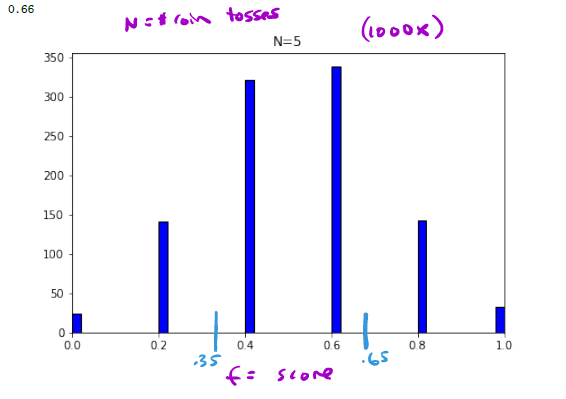
\includegraphics[width=140mm]{2.png}
	\caption{Score histogram for $1000$ coin tosses carried out $N=5$ times}
\end{figure}

\begin{figure}[H]
	\centering
	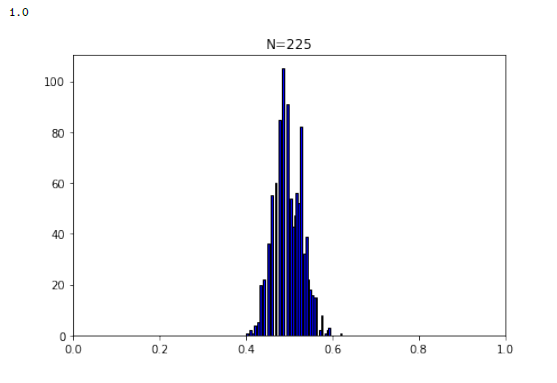
\includegraphics[width=140mm]{3.png}
	\caption{Score histogram for $1000$ coin tosses carried out $N=225$ times}
\end{figure}

If $N = \infty$, the histogram will look like the delta function centered at $0.5$. \\

Regarding example one, this is a bit different compared to this example. Behaviour as something approaches infinity and behaviour at infinity are two different things. In example one, as $k\to\infty$, the probability of getting \textit{exactly} $k$ heads and tails will approach zero. Any finite $k$ is far from infinity. Now back to the example we are discussing right now, when $N = \infty$ the fraction is exactly $0.5$ and, of course, there is the exact match in heads and tails, both infinite.

\subsection{Probability for Binomial Random Variable*}

\textit{This section is optional.} \\

Suppose you want to calculate the probability of getting a certain combination of heads and tails from an unfair coin. It depends on whether the order matters or not.

\begin{texample}
	Consider an unfair coin, let the probability of getting $H$ on a single toss be $0.6$ and the probability of getting $T$ is $0.4$. Find (1) the probability of obtaining the sequence $THHTTTHT$ (exactly, in this order) (2) the probability that a sequence of eight coin tosses would have $5$ tails and $3$ heads in any order. \\
	
	(1) Coin toss events are independent of each other. The probability will be calculated as follows $0.4\cdot0.6\cdot0.6\cdot0.4\cdot0.4\cdot0.4\cdot0.6\cdot0.4=0.6^30.4^5=0.00221$. By symmetry, this is the same as the probability of getting the sequence $TTTTTHHH$ (or any other arrangements involving $3$ heads and $5$ tails) in exact order. \\
	
	(2) The probability of getting $5$ tails and $3$ heads in any order can be calculated using the addition law for disjoint events:
	
	\begin{align*}
		P(\text{$3$ heads})&=P(\{THHTTTHT\}) + P(\{THTHTTTH\}) \\
		&\quad+ P(\{TTHTHHTT\}) + \cdots \\
		&\quad + P(\{\text{other arrangements of $3H$ and $5T$}\})
	\end{align*}
	
	In this case, we need to find the number of ways to permute $5$ tails and $3$ heads which is given by $\binom{8}{3}=56$. Using our answer to (1), the probability is therefore:
	
	$$P(\text{$3$ heads})=56\cdot0.00221=0.12386$$
	
	This example presents the basic intuition for how to calculate probabilities for binomial random variables.
\end{texample}

Suppose you are doing an experiment where the probability of success is $p$ and failure is $1-p$. The probability of getting exactly $k$ successes out of $n$ trials can be calculated by the below formula:

$$P(\text{$k$ successes out of $n$ trials})=\binom{n}{k}p^k(1-p)^{n-k}$$

\begin{texample}
	Using the same unfair coin from the previous example, define a score to be (number of Heads) / (number of tosses). Find the probability that the score is between $0.4$ and $0.8$ when $N=9$ coins are tossed. What is the answer if $N$ is very large? \\
	
	To get the score between $0.4$ and $0.8$, we need to get $4$ to $7$ heads. So the probability is
	
	\begin{align*}
		P(\text{score between 0.4 and 0.8})&=P(\text{4 or 5 or 6 or 7 heads}) \\
		&= P(\text{4 heads})+P(\text{5 heads}) \\
		&\quad + P(\text{6 heads})+P(\text{7 heads}) \\
		&= \sum_{k=4}^7 \binom{9}{k}0.6^k0.4^{9-k} \\
		&= 0.8301
	\end{align*}
	
	If $N$ is very large, the probability will reach $1$.
\end{texample}

\subsection{Standard Deviation}

In the coin experiment, we noticed that as $N$ tends to infinity, the score converges to $\frac{1}{2}$. This means the larger the $N$ is more accurate the measurement is. This is reflected in the uncertainty of the measurement. This uncertainty is called ``standard deviation,'' average distance from mean. \\

One can estimate uncertainty using the 68–95–99.7 rule.

\begin{figure}[H]
	\centering
	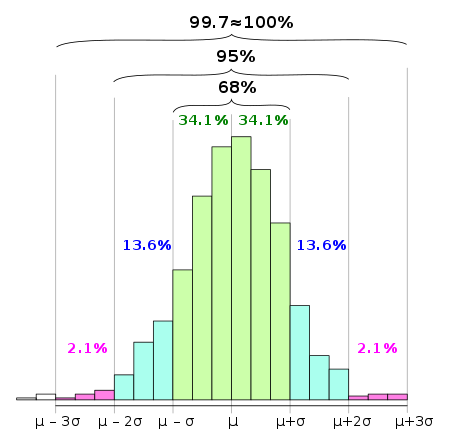
\includegraphics[width=120mm]{4.png}
	\caption{Distribution of mass in Gaussian}
\end{figure}

One standard derivation $\sigma$ left and right from mean value $\mu$ will give about $68\%$ of the overall mass. Two standard derivations left and right from the mean will give about $95\%$ of the overall mass. \\

Standard deviation squared for a single measurement $N=1$ is given by $\sigma_1^2 = \langle (x - \langle x \rangle)^2 \rangle$ where $x$ are all possible outcomes of a single measurement and $\langle x \rangle$ is theoretical mean which is given by:

$$\langle x \rangle= \lim_{N\to\infty}\frac{1}{N}\sum_{i=1}^N x_i$$

\begin{texample}
	Find $\sigma_1^2$ for a dice roll experiment. \\
	
	There are six possible outcomes for this experiment which are $x=1, 2, 3, 4, 5, 6$. The mean of these outcomes is $\frac{1+2+3+4+5+6}{6}=3.5$. The standard deviation squared is given by
	
	$$\sigma_1^2 = \frac{1}{6} \sum_{x=1}^6 \left( x - 3.5 \right)^2 = 2.91667$$
\end{texample}

The standard deviation squared after $N$ measurements is given by $\sigma_N^2 = \langle (x_N - \langle x \rangle)^2 \rangle$ where $x_N$ is the mean of $x$ after $N$ measurements:

$$x_N = \frac{1}{N}\sum_{i=1}^N x_i$$

\begin{texample}
	Consider a coin tossing experiment, find standard deviation after two measurements. \\
	
	The possible outcomes after two measurements are $HH$, $TH$, $HT$, and $TT$.
	
	\begin{align*}
		\sigma_2^2 &= \left\langle \left( \frac12 \sum_{i=1}^2 x_i - \langle x \rangle \right)^2 \right\rangle  = \left\langle  \left(\frac12 \left(x_1 + x_2 \right)  - \langle x \rangle \right)^2\right\rangle \\
		&= \frac14 \left[ \left(\frac12(0+0)-0.5\right)^2 + \left(\frac12(0+1)-0.5\right)^2 \right. \\
		&\phantom{-} + \left. \left(\frac12(1+0)-0.5\right)^2 +\left(\frac12(1+1)-0.5\right)^2 \right] = \frac18
	\end{align*}
	
	We have $\sigma_2 = \frac{1}{\sqrt{8}}$. The standard deviation for a single measurement is $\sigma_1=\sqrt{\frac12 \left( (0-0.5)^2+(1-0.5)^2 \right)}=\frac{1}{2}$. So $\sigma_2 = \frac{\sigma_1}{\sqrt{2}}$.
\end{texample}

\begin{texample}
	Show that $\sigma_N^2=\frac{\sigma_1^2}{N}$.
	
	\begin{align*}
		\sigma_N^2 &= \langle (x_N - \langle x \rangle)^2 \rangle \\
		&= \left\langle \left(\left( \frac{1}{N}\sum_{i=1}^N x_i \right) - \langle x \rangle\right)^2 \right\rangle \\
		&= \left\langle \frac{1}{N^2}\left( \sum_{i=1}^N x_i \right)^2 - \frac{2 \langle x \rangle}{N} \left( \sum_{i=1}^N x_i \right) + \langle x \rangle^2 \right\rangle
	\end{align*}
	
	We will use the following fact that $\left( \sum_{i=1}^N x_i \right)^2 = \sum_{i=1}^N \sum_{j=1}^N x_i x_j$ and $\langle x_i \rangle = \langle x \rangle$ to simplify the equation further:
	
	\begin{align*}
		&= \left\langle \frac{1}{N^2}\left( \sum_{i=1}^N \sum_{j=1}^N x_i x_j \right) - \frac{2 \langle x \rangle}{N} \left( \sum_{i=1}^N x_i \right) + \langle x \rangle^2 \right\rangle \\
		&= \frac{1}{N^2}\left( \sum_{i=1}^N \sum_{j=1}^N \left\langle x_i x_j \right\rangle \right) - \frac{2 \langle x \rangle}{N} \left( \sum_{i=1}^N \left\langle x_i \right\rangle \right) + \left\langle \langle x \rangle^2 \right\rangle \\
		&= \frac{1}{N^2}\left( \sum_{i=1}^N \sum_{j=1}^N \left\langle x_i x_j \right\rangle \right) - \frac{2 \langle x \rangle}{N} N\langle x \rangle + \langle x \rangle^2 \\
		&= \frac{1}{N^2}\left( \sum_{i=1}^N \sum_{j=1}^N \left\langle x_i x_j \right\rangle \right) - \langle x \rangle^2 \\
		&= \frac{1}{N^2}\left( \sum_{i=1}^N \left\langle x_i^2 \right\rangle + \sum_{i \ne j} \left\langle x_i \right\rangle \left\langle x_j \right\rangle \right) - \langle x \rangle^2 \\
		&= \frac{1}{N^2}\left( \sum_{i=1}^N \left\langle x^2 \right\rangle + \sum_{i \ne j} \left\langle x \right\rangle^2 \right) - \langle x \rangle^2 \\
		&= \frac{1}{N^2}\left( N \left\langle x^2 \right\rangle + (N^2-N) \left\langle x \right\rangle^2 \right) - \langle x \rangle^2 \\
		&= \frac{1}{N} (\left\langle x^2 \right\rangle -\left\langle x \right\rangle^2)
	\end{align*}
	
	We have $\sigma_1^2 = \langle (x- \langle x \rangle)^2 \rangle = \langle x^{2} - 2x\langle x \rangle + \langle x \rangle^2 \rangle = \langle x^2 \rangle - 2 \langle x \rangle \langle x \rangle + \langle x \rangle^2=\langle x^2 \rangle - \langle x \rangle^2$, so the final result is $\sigma_N^2=\frac{\sigma_1^2}{N}$.
\end{texample}

Since it doesn’t matter how you group the experiments or number of trials, the std error of the mean for 10 coin tosses 100 times is the same as that for 100 coin tosses 10 times.

\begin{texample}
	Show that the standard deviation of $100$ experiments of $10$ coin flips is the same as that of $10$ experiments of $100$ coin flips.
	
	\begin{align*}
		\sigma (\text{$100$ experiments of $10$ coin flips}) = \frac{\sigma_{10}}{\sqrt{100}}=\frac{\sigma_1}{\sqrt{100}\sqrt{10}} \\
		\sigma (\text{$10$ experiments of $100$ coin flips}) = \frac{\sigma_{100}}{\sqrt{10}}=\frac{\sigma_1}{\sqrt{10}\sqrt{100}}
	\end{align*}
\end{texample}

In the coin toss experiment, we can approximate the standard deviation of scores using $\sigma_N \propto \frac{1}{\sqrt{N}}$. The score now is given by $f=\frac{1}{2} \pm \sigma_N = \frac{1}{2} \pm \frac{1}{\sqrt{N}}$. As $N\to\infty$, the score is $f=\frac{1}{2}$, as expected.

\begin{texample}
	A box, divided into two identical parts by a partition with a small hole in it, has 1 mole of ideal gas in it. After a while, the hole is plugged up, and the number of atoms on each side of the partition is counted. How large (roughly) would you expect the difference between the two counts to be within? Recall Avogadro's number $N_A=6\times10^{23}$. \\
	
	An ideal gas is a kind of gas where non-interacting particles each acts independently of the others. This is like the coin-flipping experiment we discussed earlier. The amount of atoms on one part of the box is given by:
	
	$$N_A \left(\frac{1}{2} \pm \frac{1}{\sqrt{N_A}}\right) = \frac{N_A}{2} \pm \sqrt{N_A}$$
	
	We see that the uncertainty given by $\sigma=\sqrt{N_A}$ which corresponds to the order of the magnitude of about $10^{12}$ atoms.
\end{texample}
